\section{Friction}

\begin{multicols}{2}


\section*{Concept of Friction}


\subsection{Useful Friction}

\begin{center}
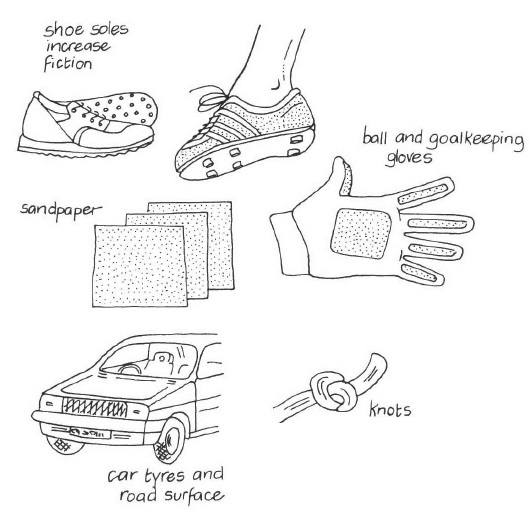
\includegraphics[width=0.5\textwidth]{./img/vso/useful-friction.jpg}
\end{center}

\subsection{Pencil Roller}

\begin{center}
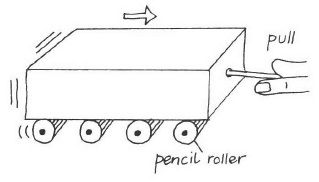
\includegraphics[width=0.4\textwidth]{./img/vso/pencil-roller.jpg}
\end{center}

\begin{description*}
%\item[Subtopic:]{}
\item[Materials:]{Pencils, \nameref{sec:spring-balance}, matchbox/block of wood}
%\item[Setup:]{}
\item[Procedure:]{Use a spring balance to pull a matchbox or block of wood across a table at constant speed. Then repeat by pulling the object across a row of pencils. Compare the results of the spring balance.}
%\item[Hazards:]{}
%\item[Questions:]{}
\item[Observations:]{The spring balance shows a lower force reading when rolled on pencils.}
\item[Theory:]{Rollers reduce friction compared to sliding along a table surface. Because the object is pulled at constant speed, the force on the spring balance is equal to the force of friction acting on the object.}
%\item[Applications:]{}
%\item[Notes:]{}
\end{description*}

%==================================================================================================%

\section*{Laws of Friction}


\subsection{Factors Affecting Friction}

\begin{center}
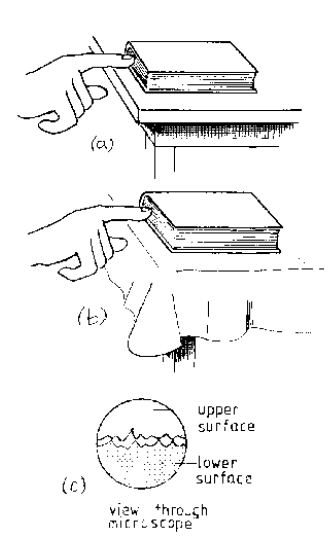
\includegraphics[width=0.49\textwidth]{./img/source/friction-factors.png}
\end{center}

\begin{description*}
%\item[Subtopic:]{}
\item[Materials:]{Books of various sizes, table, cloth}
%\item[Setup:]{}
\item[Procedure:]{Pull a book on a bare surface and then on a piece of cloth. Repeat for a sheet of paper and a thick book of the same page size.}
%\item[Hazards:]{}
%\item[Questions:]{}
\item[Observations:]{It is harder to pull the objects on a cloth surface than on a bare table. Heavier objects are more difficult to pull.}
\item[Theory:]{Friction depends on the nature of the two surfaces in contact. It is directly proportional to the normal force ($R$) between the two surfaces in contact ($F_f=\mu R$). It is independent of the surface area of contact and the relative speed of the objects.}
%\item[Applications:]{}
%\item[Notes:]{}
\end{description*}

\columnbreak

%==================================================================================================%

\section*{Coefficient of Friction}


\subsection{Limiting Friction}

\begin{center}
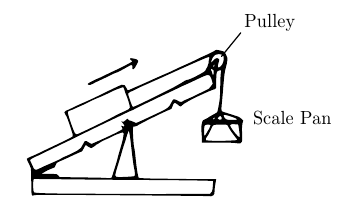
\includegraphics[width=0.5\textwidth]{./img/limiting-friction.png}
\end{center}

\begin{description*}
%\item[Subtopic:]{}
\item[Materials:]{2 wooden boards 60 cm $\times$ 2 cm, wood block 10 cm $\times$ 5 cm $\times$ 2 cm, nails, hinge, \nameref{sec:masses}, string, pulley, protractor, plastic water bottle}
\item[Setup:]{Connect the boards together at one end with a hinge and nails. Attach a pulley to the free end of one board. Prop up this end to create an inclined plane. Cut the bottom 5 cm off of the water bottle to make a scale pan.}
\item[Procedure:]{Record the mass of a wooden block using a spring balance or beam balance and calculate its weight $W$. Measure the angle of incline $\theta$ between the two boards using a protractor. Attach the string to the block on one end, and the scale pan on the other. Add masses to the scale pan until the block just starts to move. Record the mass added and calculate its weight. Repeat for various angles of the incline.}
%\item[Hazards:]{}
\item[Questions:]{Calculate the limiting friction and the coefficient of static friction $\mu_s$ of the block.}
\item[Observations:]{The mass (and thus weight) required to move the block increases as the angle increases.}
\item[Theory:]{The weight added to the scale pan is equal to the limiting friction $F_f$ of the block. This is the minimum force necessary to move the block. To find $\mu_s$, we use the relation $F_f=\mu_s R$, where $R$ is the normal force. It can be seen through trigonometry that $R=W\cos{\theta}$ ($W$ is the weight of the block). Thus, $\mu_s=\cfrac{F_f}{W\cos{\theta}}$.}
%\item[Applications:]{}
%\item[Notes:]{}
\end{description*}

\vfill
\columnbreak

%==================================================================================================%

\section*{Applications of Friction}


\subsection{Friction Produces Heat}

\begin{center}
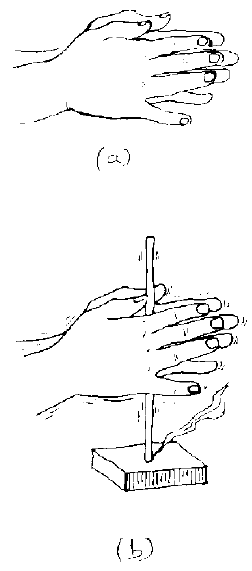
\includegraphics[width=0.4\textwidth]{./img/source/friction-heat.png}
\end{center}

\begin{description*}
%\item[Subtopic:]{}
\item[Materials:]{Stick, piece of wood, matches}
%\item[Setup:]{}
\item[Procedure:]{Rub your hands together and feel the heat produced. Rub a stick into a piece of wood until it begins to smoke and burn. Strike a match against a rough surface to light it.}
%\item[Hazards:]{}
%\item[Questions:]{}
%\item[Observations:]{}
\item[Theory:]{Friction produces heat which can start a fire if great enough.}
%\item[Applications:]{}
%\item[Notes:]{}
\end{description*}

\vfill
\columnbreak

\subsection{Lubrication}

\begin{center}
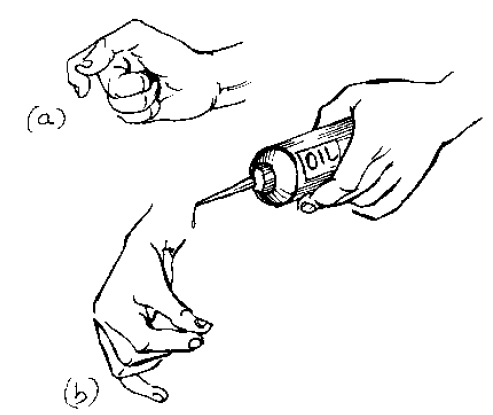
\includegraphics[width=0.4\textwidth]{./img/source/lubrication.png}
\end{center}

\begin{description*}
%\item[Subtopic:]{}
\item[Materials:]{Cooking oil/margarine}
%\item[Setup:]{}
\item[Procedure:]{Rub your fingers together. Then place a drop of oil on your thumb and repeat rubbing.}
%\item[Hazards:]{}
\item[Questions:]{How can friction be reduced in machinery and other moving parts?}
%\item[Observations:]{}
\item[Theory:]{Oil is a common lubricant used to reduce friction between two surfaces.}
\item[Applications:]{Bearings, auto parts, bicycles, gears, etc.}
%\item[Notes:]{}
\end{description*}

\subsection{Water as a Lubricant}

\begin{center}
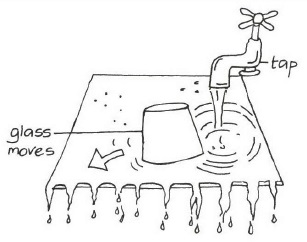
\includegraphics[width=0.4\textwidth]{./img/vso/water-lubricant.jpg}
\end{center}

\begin{description*}
%\item[Subtopic:]{}
\item[Materials:]{Sheet of glass, drinking glass, water}
%\item[Setup:]{}
\item[Procedure:]{Cover the sheet of glass with water. Leave a little water in the drinking glass and then invert it.}
%\item[Hazards:]{}
%\item[Questions:]{}
\item[Observations:]{The glass floats on a cushion of air and water like a hovercraft.}
\item[Theory:]{The coefficient of friction between glass and water is lower than that of glass and glass. Thus, the water acts as a lubricant and a glass surface is able to move across the surface of water more easily than across another surface of glass.}
%\item[Applications:]{}
%\item[Notes:]{}
\end{description*}

%==================================================================================================%


\end{multicols}

\pagebreak